%; whizzy chapter
% -initex iniptex -latex platex -format platex -bibtex jbibtex -fmt fmt

%   Pdf作成手順
% dvipdfmx debianmeetingresume200507.dvi


%     Tokyo Debian Meeting resources
%     Copyright (C) 2006 Junichi Uekawa

%     This program is free software; you can redistribute it and/or modify
%     it under the terms of the GNU General Public License as published by
%     the Free Software Foundation; either version 2 of the License, or
%     (at your option) any later version.

%     This program is distributed in the hope that it will be useful,
%     but WITHOUT ANY WARRANTY; without even the implied warranty of
%     MERCHANTABILITY or FITNESS FOR A PARTICULAR PURPOSE.  See the
%     GNU General Public License for more details.

%     You should have received a copy of the GNU General Public License
%     along with this program; if not, write to the Free Software
%     Foundation, Inc., 51 Franklin St, Fifth Floor, Boston, MA  02110-1301 USA

%この資料はA3用紙に両面印刷で印刷する予定

\documentclass[mingoth]{jsarticle}
\usepackage[dvipdfmx]{graphicx}
\usepackage{fancybox}
\usepackage{longtable}

%%gotom
\usepackage{ascmac}	% 囲み (screen,itembox)
\usepackage{fancyvrb}   % 囲み Verbatim のために必要
%%

\usepackage[dvipdfmx]{hyperref}
\usepackage{url}

\AtBeginDvi{\special{pdf:tounicode EUC-UCS2}}

% とりあえずcommandline環境を定義。入出力についてはcommandline環境を活用
%する
\newenvironment{commandline}%
{\VerbatimEnvironment
  \begin{Sbox}\begin{minipage}{12cm}\begin{tiny} \begin{BVerbatim}}%
{\end{BVerbatim}\end{tiny}\end{minipage}\end{Sbox}
  \setlength{\fboxsep}{8pt}\fbox{\TheSbox}}



% 三択問題用
\newcounter{santakucounter}
\newcommand{\santaku}[4]{%
\addtocounter{santakucounter}{1}

\nopagebreak 問題\arabic{santakucounter}. 
#1\\
\nopagebreak□ A #2\\
\nopagebreak□ B #3\\
\nopagebreak□ C #4
\pagebreak[1]
\hspace{1cm}
\\

}

\newcommand{\emptyspace}{(\underline{\hspace{1cm}})}



\newcommand{\subsubsubsection}[1]{%
\vspace{1zw}{\bf #1}\\}


% sectionをセンタリングする
\makeatletter
  \renewcommand{\section}{\@startsection{section}{1}{\z@}%
    {\Cvs \@plus.5\Cdp \@minus.2\Cdp}% 前アキ
    {.5\Cvs \@plus.3\Cdp}% 後アキ
    {\normalfont\Large\headfont\raggedright\centering}} % style
\makeatother

% section の代わりの環境
\newcommand{\dancersection}[2]{%
\newpage
東京エリアDebian勉強会 2005
\hrule
\vspace{0.5mm}
\hrule
\hfill{}
\includegraphics[width=3cm]{image200502/openlogo-nd.eps}\\
\vspace{-4cm}
\begin{center}
  \section{#1}
\end{center}
\hfill{}#2\hspace{3cm}\space\\
\hrule
\hrule
\vspace{1cm}
}




%% for gotom
\newenvironment{gdescription}%  
{%
   \begin{list}{}% 見出し記号/直後の空白を調節
   {%
      \setlength{\itemindent}{0mm}
      \setlength{\leftmargin}{45mm}%  左のインデント
      \setlength{\rightmargin}{0zw}% 右のインデント
      \setlength{\labelsep}{4mm}%    黒丸と説明文の間
      \setlength{\labelwidth}{4cm}%  ラベルの幅
      \setlength{\itemsep}{0em}%     項目ごとの改行幅
      \setlength{\parsep}{0cm}%      段落での改行幅
      \setlength{\listparindent}{0cm}% 段落での一字下り
      \let\makelabel\gdescriptionlabel
   }
}{%
   \end{list}%
}
\newcommand*\gdescriptionlabel[1]{\hspace\labelsep\normalfont\bfseries #1}
%%

\begin{document}

\begin{titlepage}

% 毎月変更する部分
\title{
 第6回 東京エリア Debian 勉強会\\事前資料
\footnote{機密レベル public: 一般開示可能}}
\date{2005年7月2日}
\author{Debian勉強会会場係 上川 純一\thanks{Debian Project Official Developer}} 
\maketitle

\end{titlepage}

\newpage
\tableofcontents

\dancersection{Introduction To Debian 勉強会}{上川 純一}

今月のDebian勉強会へようこそ。
これからDebianのあやしい世界に入るという方も、すでにどっぷりとつかってい
るという方も、月に一回Debianについて語りませんか?

目的として下記の二つを考えています。

\begin{itemize}
 \item メールではよみとれない、もしくはよみとってられないような情報を情
       報共有する場をつくる
 \item まとまっていないDebianを利用する際の情報をまとめて、ある程度の塊と
       して出してみる
\end{itemize}

また、東京にはLinuxの勉強会はたくさんありますので、Debianに限定した勉強
会にします。Linuxの基本的な利用方法などが知りたい方は、他でがんばってくださ
い。
Debianの勉強会ということで究極的には参加者全員がDebian Packageを
がりがりと作りながらスーパーハッカーになれるような姿を妄想しています。

Debianをこれからどうするという能動的な展開への土台としての空間を提供し、
情報の共有をしたい、というのが目的です。
次回は違うこと言ってるかもしれませんが、御容赦を。

\subsection{講師紹介}

\begin{itemize}
 \item{gotomさん} Debianのglibcとかをやってます。
 \item{上川 純一} 宴会の幹事です。
      Debian Developerです。
      元超並列計算機やっていて、
      今は音楽関係とか、気づいたらcannaとか。
      あと、pbuilderや、libpkg-guideなどを通して、Debianの品質向上を目指してます。
\end{itemize}

\subsection{事前課題紹介}

今回の事前課題は
「いままでtoolchainをつかってみて/今後toolchainに期待すること」
というタイトルで200-800文字程度の文章を書いてください。
というものでした。
その課題に対して下記の内容を提出いただきました。

\subsubsection{makoyukiさん}

えー、すいません、当方、そもそも「toolchain」といわれて何のことかわかり
ませんでした。
大体「開発環境一式」とかかなぁ?という感じだったのですが、正確に理解して
いるかわかりません。

んで、仮にそうだとして、ある程度のコンパイルとかはしていても、当方コード
書きではまったく無い上、少なくともDebianにおいては一度も手動でソースコー
ドからコンパイルしたことがありませんし、プログラミング周りのことについて
はド素人なのでド素人なりのことを書いてみます。

開発環境であるという前提で書きますが…
正直に包み隠さず言いますと、当方は実際のところプログラミングっぽいことが
したくないからDebianを使っています。コードは書きたくないのです。
万が一それが楽しいと思うことがあれば今後絶対にやらないということはありま
せんが、少なくとも今、私がやりたいのはプログラミングではありません。
なので、「toolchainを使う」ということは、当面ないと思うのです。いままで
も。そしてこれから当分の間は。

勿論、勉強にもなりますし、理解を深める一助にもなるでしょうから、それにつ
いての勉強をしたいとは思います。その上で、限度はあるにせよ、ドキュメント
の充実、ツールやインターフェースの充実により、レベルは下げずに敷居を下げ
るものであって欲しいという浅はかな望みはありますが、それはなんとなく今回
のお題にはそぐわない気もします。

そもそもがtoolchainが何のことか理解していないかもしれませんので完全にハ
ズしているかもしれませんがご勘弁を。


\subsubsection{澤田さん}

toolchainに期待すること、ということでいろいろ妄想してみた。

まず現実的なもの。最適化は結構ブラックボックスなイメージがあるの 
で、最適化を行ったときにどの部分にどんな最適化を施したのか、逆に 
ここはなんで最適化をかけなかったのか(時間と空間のトレードオフと 
か)、最適化をかけることでどんな効果が得られるのかのログがあると 
いいなと思った。

もうひとつまあまあ現実的なもの。リンク時にどのライブラリをリンク 
しないといけないのか考えるのが面倒なので、ライブラリが 
exportしているシンボルを保存しておき、リンク時に参照する機能があ 
るといいなと思った。この場合、どのライブラリを使っているかわから 
なくなってしまうので、デフォルトオフで--library-auto- 
detectとかいうオプションがあるといいだろうか。

次に実現できるかよくわからないもの。コンパイル時にはinline 
展開なるものがあるわけだが、リンク時(共有ライブラリ使ってる場合 
はロード時)にもinline展開してくれるとうれしいことがあるか 
もしれないと思った。

最後にかなり非現実的なもの。最適化を行う際に一番問題なのはやはり 
どの最適化オプションを使えばいいのかわからないということであろ 
う。これを解決する方法として、こんなコードに対してはこんな最適化 
が有効だったというデータベースを構築し、最適化時にそれを参照、実 
行してデータベースに反映とかすると何かができるのではないかと思っ 
た。

\subsubsection{KATOさん}


Toolchain = glibc/binutils/gcc ということで,
glibc はもちろん, gcc, binutilsを普通に使ってきましたが
今まで特に「toolchain」という形で特に意識したことはありませんでした.
ですから「使ってみて」といって実は何を書いたらよいのか良くわかりません.
Toolchain の構成要素はそれそれ互いに密接に関連していて,
うまく連携がとれている必要があると思うのですが,
今後に期待するのは, (興味のない人は)toolchainのことを特に意識しないでも
安定してDebianを使い続けられるようにきちんと連携たとれた状態に
メンテナンスされているように, ということです.

\subsubsection{中島 清貴さん}

なかなかとても良い。このような使いやすいシステムがあったとは今まで全然知らなか
った。ぜひわたしの友人、知人その他の世話になった方々に使ってみてもらいたい。と
心底思います。toolchainを知って本当に良かったです。もし、まだ使っていないのな
ら、すぐに使うべきです。断言します。とてもおすすめです。これは絶対に使うべきで
す。私がこのようなシステムを使えるということは、なによりの喜びであり使ってみて
本当に感激いたしました。これは使わなければ大損です。

\subsubsection{Hidetaka Iwaiさん}
今回のお題は toolchain とのことですが、個人的には toolchain に関して特
に要望等はありません。debuan 2003 年夏号に顛末が書いてあった VIA C3 で
の libssl 動作問題のように、glibc の upstream maintainer 達や RedHat
等他の distribution の人々と協力関係を保って今後もメンテされていけば素
晴しいのではないかと思います。強いて言えば、toolchain 単独の問題ではな
いのですが、auto builder や pbuilder, dpkg-cross と協調して package を
cross compile できるようになれば、速くて安価な x86 マシンを buildd と
して投入できて、遅い buildd しかない architecture (m68k等)の security
update 等が速くなって皆幸せになれるような気がします。

\subsubsection{Nobuhiro Iwamatsuさん}

\begin{enumerate}
 \item  linuxのカーネルヘッダが必要なのはどうかと思う。
  (BSDとかはどうやってるんだろう?)

 \item  toolchain は アーキテクチャによって gcc と glibc , binutils
のバージョンの組み合わせで動いたり動かなかったりするのが問題と
思う。
しかし、Debianではサポートされているアーキテクチャで全て同じ組み
合わせというのがすばらしい。

 \item  コンパイラがコンパイルできても動くとは限らないのが問題だと
思う。Debianでも毎回テストユニットを使ってテストしてからuploadしてる
んですか?

 \item  SuperHサポートしてください。
\end{enumerate}


\subsubsection{上川}

etchにむけてg++のtransitionがあるらしい。
ABIがまた変わるとのこと。
gcc 3.0になるときに「これで最後だから」といってみておきながら、また浮気
するのですか?
あぁ。。。

woodyからsargeにあがる際に、c++のABIが一旦変更になっています。
アップグレードの際にこまったりしませんでしたか?

%%% trivia quiz
\dancersection{Debian Weekly News trivia quiz}{上川 純一}

ところで、Debian Weekly News (DWN)は読んでいますか?
Debian 界隈でおきていることについて書いているDebian Weekly News.
毎回読んでいるといろいろと分かって来ますが、一人で読んでいても、解説が少
ないので、
意味がわからないところもあるかも知れません。みんなでDWNを読んでみましょう。

漫然と読むだけではおもしろくないので、DWNの記事から出題した以下の質問にこたえてみてください。
後で内容は解説します。

\subsection{2005年24号}
6月14日版です。

\santaku{Aliothが新しいサーバに移動するということが各ユーザ宛のダイレク
トメールで出た。Branden RobinsonがAliothのアナウンスメールについてコメントを出
した。その主旨は。
}{匿名で各ユーザにメールを出すのではなく、debian-devel-announceに出そう、
さらに誰が出したのかを明確にして出そう}{メールは信頼できないプロトコルな
のでWEBページに掲示したらよいだろう}{SMTPより、SNMP トラップのほうがみんな気づく}

\santaku{Andreas Barthはetchに向けてリリースポリシーについてどういう変更が必要だと説
明したか}{ダメな人禁止}{ダメなコード禁止}{共有ライブラリはダイナミックにリンクすべきであり、ソースコード
をコピーするのは禁止しよう。}

\santaku{etchにむけてc++のABIが変更になるため、Matthias Klose は何を宣言
したか}{C++でかいたプログラムの粛正}{とりあえず今C++のライブラリであたらしいABIバージョンのものにつ
いてはアップロードしないようにフリーズする}{javaの利用禁止}

\santaku{Debconfでの講演の予定の組み方について今回はどういうこころみ
がなされたか}{意志決定方法としてさいころを導入してみた}{
参加者の都合が悪い日をできるだけ選んだ}{参加したい講演の投票をおこない、参加者ができるだけ参加
できるようにスケジューリングをする}

\santaku{Scott James Remnant曰く、dpkg 1.13で新しく追加されたアーキテク
チャ変数名は}{DPKG\underline{ }HOST\underline{ }ARCH\underline{ }OS}{
DEBIAN-ARCHITECTURE}{uname -a }

\santaku{Roberto Sanchezの作成したFAQには何がかいてあるか}
{Debianパッケージをインストールする方法がかいてある}{
Debianパッケージをカスタマイズしてビルドする手順がかいてある}{Debianメン
テナを招集する方法がかいてある}

\santaku{selinuxの進捗についてはどうなっているか}{coreutilsなどのパッケー
ジがlibselinux1に依存するようになってきた}
{NSAの陰謀であることが判明したので排除}{もうほとんどのユーザがSELINUXを
使うようになった}


\subsection{2005年25号}
6月21日版です.

\santaku{OskuroがGNOMEについて宣言したのは何か}{今後はKDEに移行する}{Gnome 2.10がunstableに
入った}{GNOME3がもうすぐリリース}
\santaku{woodyからsargeにアップグレードするのにもっとも大きい問題は何か}
{相互に依存するような依存関係があるパッケージのアップグレード}{
woodyでは存在したけどsargeで消えたパッケージの処理}{etchに無いパッケージ}

\santaku{Aurelien JarnoがBSD移植版について報告した問題は}
{GNU Hurdについてはもうあきらめたので考えなくて良い}{
FreeBSDについてはもうあきらめた。
}{libselinux1に依存するパッケージは、selinuxがlinuxのみなので、Linux
のみでリンクするようにしてほしい}

\santaku{Bill Allombertがmenuについて報告したのは}{menuのセクション
の部分については国際化できるようになった}{menuはもう使われていないので廃
止する}{対応するWindow Managerが増えた}

\santaku{矢吹さん曰く大阪でなにかあるらしい、何?}{10月にmini Debian
Conferenceを開催する }{9月にたこやきはやぐい競争}{阪神優勝祈念会}

% \santaku{}{}{}{}
% \santaku{}{}{}{}
% \santaku{}{}{}{}
% \santaku{}{}{}{}

\subsection{2005年26号}
6月28日版です.

\santaku{Debian Policy CommitteeをBranden Robinsonが発表しました。チェア
マンは誰?}{Manoj Srivastava}{Andreas Barth}{Matt Zimmerman}
\santaku{Andreas Barth は etch向けのリリースポリシーを発表しました。
そのなかにあった記述は}{debian/changelog や debian/control ファイルを通
常のビルド処理で変更することを禁止する}{
二年以内にはリリースしない
}{パッケージの数は10万を越えることを目標にする}
\santaku{XML形式のインタプリタ言語CYBOPをDebianに含める場合、プログ
ラムはどこにおいたらよい?}{ユーザが実行できるなら/usr/bin以下、
ライブラリモジュールなどなら/usr/share/cybopのような場所を指定する}
{/srv}{
XMLベースの言語なんてとんでもない}
\santaku{cogitoというプログラムとgitというプログラムが、/usr/bin/gitを両
方保持していて、conflict: していたことに関しての反論は}{
/usr/bin/git の機能が全く違う}{
/usr/bin/gitはGNUの商標です
}{cogitoの/usr/bin/gitが一番よく使われているからGITのgitなんか不要}

\santaku{openafsパッケージは全アーキテクチャではビルドできない。
しかし、Architecture: allのパッケージがあるために、各アーキテクチャでビ
ルドが試行されてしまう。
そのような状況を表現する最良の方法は何?
}{Build-Depends: type-handlingでアーキテクチャを指定}{
Packages-arch-specific を使う
}{builddのメンテナに個人的にメールを送る}
\santaku{tetexがすでにあるのにTeXliveをパッケージする理由としては}{
たくさんのTeXパッケージがあり、年に一回リリースしている}{
tetexは使えない}{
そこにTeXliveがあるから}
% \santaku{}{}{}{}
% \santaku{}{}{}{}
% \santaku{}{}{}{}
% \santaku{}{}{}{}
% \santaku{}{}{}{}
% \santaku{}{}{}{}

%\subsection{2005年27号}
% \santaku{}{}{}{}

\dancersection{最近のDebian関連のミーティング報告}{上川 純一}

\subsection{東京エリアDebian勉強会5回目報告}


前回開催した第5回目の勉強会の報告をします。

DWNクイズを実施しました。
	    今回は3週間分だったので、分量がすくなかったかな。

えとーさんがupdate-alternativesとdsysについて説明しました。
	    update-alternativesが 実はroot権限がなくても使えるようになっていたり、
	    新しい発見がありました。
	    dsysについては、alternativesのDescription(説明文)というものがないので
	    その情報が欲しい、さらに国際化するには何が必要だろう、という話題が出ました。

	    武藤さんがdebian-installerの構造について話をしました。
	    国際化はまだetchにむけて改善できるだろう、ということです。
	    udebをつかっていたり、annaをつかっていたり、
	    cdebconfを使っているところとか。
	    1st-stageと2nd-stage があって、全然違うとか。
	    インストーラが動いているときにはDEBCONF\underline{ }PRIORITYはHIGHなのに
	    インストール後はMEDIUMに強制変更するためいろいろとひずみがでているとか。
	    なお、自動認識されないハードウェア情報については、
	    バグレポートが重要なので、lspci, lspci -n
	    の出力とともにおくってくださいとのこと。
	    lspci -nの出力はしらなかったけど便利。

	    GPGKeysigning partyをしました。
	    キーサイニングに参加するのは
	    10人なので、あまり時間かからないかなぁ、と思ったら30分くらいかかってしまいました。

はなの舞で宴会、デニーズでデザート。

\dancersection{Debian ツールチェインと glibc, linux-kernel-headers パッ
ケージ}{後藤正徳 \footnote{GOTO Masanori, gotom@debian.org, Debian
Project, 2005-07-02}}
\label{sec:gotom}
%% gotomさんの記事はここから

\subsection{はじめに}

   先ほどリリースされた Debian sarge では 11 ものアーキテクチャをサポートしている。
   これら異なるアーキテクチャが同時に使い物になるためには、当然各アーキ
   テクチャ用バイナリを生成するツールチェインも十分整備されていなけれ
   ばならない。

   本文書では、ツールチェインとは何かを簡単に紹介した後、筆者がメンテナン
   スしているglibc, linux-kernel-headersパッケージに関して説明を行う。

\subsubsection{ツールチェインとは}

   ツールチェイン (toolchain) という用語に正確な定義があるわけではないが、一般にマシン
   ネイティブなバイナリを生成・加工するための一連のツール群を指す
   ことが多い。
   本節では、まず Debian での代表的なツールチェインパッケージを紹介する。

  \subsubsection{gcc}

    GNU Compiler Collectionの略称。ツールチェインのコアパッケージであり、
    ソースコードからアーキテクチャ毎のバイナリへ変換する役割を持つ。なお、gcc 自体は
    ソースコードからアセンブラコードを出力するまでの機能しか持っておらず、そこから先のバイナリ生成部分
    は後述する
    binutils のツールを内部で呼び出している。
    現在サポートするプログラム言語としては C (gcc), C++ (g++), Java
    (gcj), Fortran (g77, g90) などが
    ある。

    Debian パッケージメンテナは Debian-gcc チーム 
    (Matthias Klose, Gerhard Tonn) であるが、事実上 Matthias (doko) 一人
    がメンテナンスを担っている。

  \subsubsection{binutils}

    binutils には、バイナリを生成・操作するツール群が入っている。例えば、
    gcc によって出力されたアセンブラコードをアセンブルしてオブジェクトコード化するアセンブラ
    as、複数のオブジェクトコードをリンクしてバイナリを生成するリンカ
    ld、オブジェクトコードを逆アセンブルしたり解析したりするツール objdump な
    どがある。

    Debian パッケージメンテナは James Troup である。最近では C++
    transition for etch に絡んで Matthias Klose が主な実作業にあたってい
    る。また、binutils の上流開発者の中でDebian 開発者も兼任している人
    物に Daniel Jacobowitz がいる。

  \subsubsection{glibc, linux-kernel-headers}

    glibc は GNU C Library の略称。
    gcc, binutils がバイナリを生成するものであるのに対し、glibc は生成し
    たバイナリ実行時に使用される C 言語ライブラリである。C 言語の関数や
    バイナリ実行時に最初に必要となる初期実行コードなどを含んでいる。
    なお、Cライブラリは実行環境に依存するため、システムによってはglibc 以外の libc が
    使用されることもある\footnote{例えば組み込み環境では GNU newlib、
    Debian netbsd-i386 では、NetBSD 用 libc など。}。

    linux-kernel-headers は glibc のうち /usr/include/linux など
    Linux カーネルソース起源のヘッダを扱うパッケージである。
    元々 libc6-dev パッケージにマージされていたが、ソースが別々であることから
    2つに分離された。

  \subsubsection{gdb}

    gdb はバイナリ実行時に、ユーザからデバッグを可能とするための機能を提供する。

    Debian パッケージメンテナは上流開発者でもある Daniel Jacobowitz であ
    る。

  \subsubsection{その他}

    その他のものとして C++ 向けライブラリである libstdc++ などがある。
    また、bfd といったバックエンドライブラリや dejagnu といったツール群が存在し
    ているが、本文書では割愛させて頂く。

\subsection{glibc, linux-kernel-headers パッケージの概要}

  \subsubsection{歴史}

    過去をひもとくと、元々 Linux の C ライブラリとしては H. J. Lu を中心に開発されていた
    libc4, libc5 が使用されていた。これはGNU C Library バージョン1をベー
    スにLinux向け改良が追加されたものであった。しかし、GNU C Library 自体も Roland McGrath, Ulrich
    Drepper, Andreas Jaeger を中心に別途開発が続けられており、
    古い libc5 に代わってより新しい現在の glibc バージョン 2 が libc6 と
    して置き換
    わる移行が行われた (libc6 transition)。

    Debian におけるglibc パッケージは、当初 Joel Klecker がメンテナンス
    していた (1999〜2000)。しかし Joel が病気で逝去したため、代って Ben
    Collins がメンテナンスを開始した (2000〜2002)。だが、やがて Ben 自身
    の興味が薄れて放置されるようになってきたため、現在のメンバから構
    成されるメンテナンスチームが組まれた(2002〜)。
    その後 Jeff Bailey, Branden Robinson, Daniel Jacobowitz を中心に古い 
    Debian パッケージから debhelper ベースへ完全に書き直され、同時に
    linux-kernel-headers パッケージがlibc6-dev パッケージから分離した 
    (2003)。現在は筆者を中心にメンテナンスが続けられている。

  \subsubsection{パッケージメンテナ}

    パッケージメンテナは Debian-glibc チーム。構成メンバは以
    下の通り。

	\begin{itemize}
	\item Ben Collins (benc) … 元 Debian Project Leader。
	      Debian/SPARC ポートメンバ。svn 開発者、Linux ieee1394 カー
	      ネルサブシステムメンテナ。
	\item GOTO Masanori (gotom) … 筆者。glibc 開発者、
	      Linux SCSI カーネルドライバメンテナ。
	\item Philip Blundell (pb) … Debian/ARM ポートメンバ。glibc を
	      含む上流 ARM ツールチェインや Linux/ARM カーネルのメンテナ。
	\item Jeff Bailey (jbailey) … Debian/GNU hurd-i386 ポートメンバ。現在 Ubuntu に
	      て ppc64 など先進的なツールチェインメンテナンスを行っている。
	\item Daniel Jacobowitz (drow) … Debian/PowerPC ポートメンバ。
	      glibc, gdb, gcc, binutils などをフルタイムでハック。最近の glibc 
	      まわりでは MIPS TLS や ARM new EABI などをアクティブに作業
	      している。
	\end{itemize}

      この他にも以下のメンバが活躍している。移植周り: Bastian Blank、
      debian-installer 関連: Colin Watson、locale: Petter Reinholdtsen,
      Denis Barbier、MIPS: Thiemo Seufer, Guido Guenther、hppa:
      Carlos O'Donell, amd64: Andreas Jochens, Goswin von Brederlow,
      ia64: David Mosberger, Randolph Chung, s390: Gerhard Tonn。

    \subsubsection{開発体制}

    開発は主に debian-glibc@lists.debian.org メーリングリストを中心に行
    われている。また、時々 IRC にて議論を行って今後の方針などを決定している。
    パッケージ管理は元々 cvs で行っていたが、現在は alioth の svn ベー
    スに切り替わっている。レポジトリは以下の通り。

	\begin{Verbatim}[frame=single]
	svn://svn.debian.org/svn/pkg-glibc/glibc-package/trunk
	svn://svn.debian.org/svn/pkg-glibc/linux-kernel-headers/trunk
	\end{Verbatim}

\subsection{glibc バイナリパッケージとその中身}

    本節では、glibc の各種バイナリパッケージとそれに含まれる
    ファイルを紹介していく。各ファイルの解説によって、
    glibc がどのような機能を提供しているかの一端が明らかになるだろう。

    ところで、パッケージの中には同じ機能を提供しているに
    も関わらずアーキテクチャによってついている名前が異なることがある。具
    体的に i386 での名前を挙げると libc6, libc6-dev, libc6-dbg, libc6-pic,
    libc6-prof, libc6-udeb がそうである。libc6 を例にアーキテクチャとパッ
    ケージ名の対応を表\ref{archname}に挙げる。
    以後では、一番親しんでいるであろう i386 での名前を使用して説明を進める。

    \begin{table}[h]
    \begin{center}
      {
	\begin{tabular}{l|l} \hline
		パッケージ名 & アーキテクチャ \\ \hline \hline
		libc6 & amd64, arm, i386, m68k, mips, mipsel, powerpc, sparc, s390, hppa, sh3, sh4, sh3eb, sh4eb	\\
		libc6.1 & alpha, ia64 \\
		libc0.3 & hurd-i386 \\
		libc1   & freebsd-i386 \\ \hline
	   \end{tabular}
	}
     \caption{呼称が変化するパッケージ名とアーキテクチャとの対応関係}
     \label{archname}
    \end{center}
    \end{table}

  \subsubsection{libc6}

    C ライブラリとダイナミックローダ等を提供。Priority: required,
    Section: base。

    sid/i386 では約9100バイナリパッケージが依存しているDebianのコアパッ
    ケージ。本パッケージは以下のファイルを含む。

    \begin{gdescription}

    \item[/lib/*.so] libc のコアとなる動的ライブラリ\footnote{動的ライ
        ブラリ (dynamic linked library) とは .so で終わる名前を持ち、
        バイナリ実行時に動的ローダ (dynamic loader) によって必要に応じてロー
        ドされるライブラリファイル。これに対し、静的ライブラリ (static linked library) 
        とは .a で終わる名前を持ち、コンパイル時にバイナリへライブラリコードを直接埋め込んでしま
        うために用いられるファイル。}。動的ローダ (i386 で
    	       は /lib/ld-linux.so.2) と libc (i386 では libc.so.6)、そ
	       して周辺ライブラリ (libm, libnss\_*, ...)を含む。スレッド
	       システムにはカーネル2.4でも動作するlinuxthreadsを採用。
    \item[/lib/tls/*.so] /lib/*.so と同様だが、TLS (Thread Local
	       Storage) が有効になり、デフォルトのスレッドシス
	       テムが規格により正しく準拠した NPTL (Native Posix Thread Library)になっている。
	       カーネル 2.6 使用時には、
	       デフォルトの /lib/*.so 動的ライブラリに代わってロードされる。
    \item[/lib/*.so.*, /lib/tls/*.so.*] 各ライブラリのバージョン番号を指
	       し示すためのシンボリックリンクファイル。
    \item[/usr/lib/gconv/*] gconv (各文字コード・エンコーディング毎に
	       用意されているコード変換 iconv モジュール) 動的ライブラリと gconv-modules (エイリアスファイル)。
    \item[/usr/lib/*] pt\_chown をインストール。
    \item[/usr/share/zoneinfo/*] コンパイル済タイムゾーンデータ。環境変数 TZ に指定され
	       たタイムゾーンに応じた時刻を返すために使用される。
    \item[/usr/bin/] 各種設定・変換・表示ツール (iconv, locale,
	       localedef, getent, getconf, catchsegv, tzselect, ldd,
	       lddlibc4, zdump, rpcinfo) をインストール。
    \item[/usr/sbin/*] 設定ツール (zic, iconvconfig, tzconfig) をインストー
	       ル。
    \item[/sbin/*] 動的ライブラリキャッシュファイル作成ツール ldconfig を
	       インストール。
    \item[/sys] sysfs のためのマウントポイント。歴史的事情により存在。
    \end{gdescription}

  \subsubsection{libc6-sparc64, libc6-s390x}

    64ビットbiarch\footnote{bi: 2つの、
    arch: アーキテクチャ。biarch とは、2つのアーキテクチャを同時に使用可能なこと。}
    向けに作成されているlibc6パッケージ。Priority: standard,
    Section: base。

    Debian sarge では
    sparc64, s390x にのみ提供されている。基本的にパッケージの中身は 
    libc6 パッケージと同等であるが、64ビット化した動的ライブラ
    リを /lib の代わりに /lib64, /usr/lib64 配下へインストールする。

  \subsubsection{libc6-i686, libc6-sparcv9, libc6-sparcv9b}

    アーキテクチャ依存で提供される最適化パッケージ。Priority: extra, Section: base。

    opt パッケージ、hwcap パッケージとも呼ばれる。
    基本的にパッケージの中身はlibc6パッケージと同等であるが、
    例えば libc6-i686 では /lib のかわりに /lib/tls/i686/cmov というディ
    レクトリの下に最適化された動的ライブラリがインストールされる。この最適化動的ライブラリ
    は、アーキテクチャが i686 以上かつカーネルが 2.6 以上でプロセッ
    サに cmov 拡張がある\footnote{cmov 拡張は、VIA C3以外の全ての 686 クラスプロセッ
    サが持っている。}場合、バイナリ実行時に自動的に使用さ
    れる。なお libc6-i686 は686用に最適
    化しているだけにとどまらず、スレッドサポートが大きく改善されて
    いるという重要な特徴がある。

  \subsubsection{libc6-dev}

    開発向けパッケージ。Priority: standard, Section: libdevel, Build-Essential。

    C, C++ での開発を行うためには必ず必要になる各種ファイルがインストー
    ルされる。本パッケージは以下のファイルを含む。

    \begin{gdescription}
      \item[/usr/include/*] ヘッダファイル一式を格納。
      \item[/usr/bin/*] gencat, mtrace, rpcgen といった開発用ツールを提供。
      \item[/usr/lib/*.a, /usr/lib/*.o] libc6 で提供される動的ライブラリのうちのいくつ
		 かが静的ライブラリ
		 としてインストールされる。また、コンパイル時に必ず静的
		 にリンクされるオブジェクトコードが含まれる。
      \item[/usr/lib/*.so] libc6 に含まれる /lib/*.so 動的ライブラリへの
		 シンボリックリンクファイル。コ
		 ンパイル用。
    \end{gdescription}

  \subsubsection{libc6-dev-sparc64, libc6-dev-s390x}

    64ビットbiarch向けに作成されているlibc6-devパッケージ。Priority: standard, Section:
    libdevel。

    Debian sarge では
    sparc64, s390x にのみ提供されている。基本的にパッケージの中身は 
    libc6-dev パッケージと同等であるが、64ビット化した動的ライブラ
    リを通常とは別パスへインストールする。
 
  \subsubsection{libc6-dbg}

    デバッグライブラリパッケージ。Priority: extra, Section: libdevel。

    libc6 や libc6-i686 パッケージで提供される動的ライブラリは
    strip されてシンボル情報が落とされているが、
    本パッケージで提供される動的ライブラリはシンボル情報も含んだものが
    /usr/lib/debug 配下にインストールされる。
    
    本パッケージは、開発時など glibc も含めた gdb デバッグを行う際に使用
    する。LD\_LIBRARY\_PATH 環境変数に /usr/lib/debug パスを
    含めてアプリを起動すると利用できる。

  \subsubsection{libc6-prof}

    プロファイルライブラリパッケージ。Priority: extra, Section: libdevel。

    libc6-dev で提供される静的ライブラリとほぼ同じだが、プロファイルオプション
    (-pg) つきでコンパイルされている。gprof を使ってアプリの性能プロファ
    イリングを行いたいときに利用する。

  \subsubsection{locales}

    国際化機能``ロケール''用データを提供するパッケージ。Priority: standard, Section: base。    

    Debian で日本語を使いたい場合には必ずインストールされている必要がある。本パッケージは以下のファイルを含む。

    \begin{gdescription}
      \item[/usr/share/locale/*] 国際化 (gettext化) した glibc の出力メッ
		 セージデータ(.po)。
      \item[/usr/share/i18n/charmaps/*] ロケールデータのうち文字コードに関するデータ。
      \item[/usr/share/i18n/locales/*] ロケールデータのうちロケール情報に関するデータ。
      \item[/usr/sbin/locale-gen] ロケールデータ生成スクリプト。
		 /etc/locale.gen に基づいてロケールデータを生成し
		 /usr/lib/locale へインストールする。
    \end{gdescription}

    元々localesパッケージには、コンパイル済のロケールバイナリデータ全て
    が含まれていたが、使いもしないロケール情報にサイ
    ズを食われることに強い反対意見があった。そこで現在は、各ユーザが 
    charmaps (ja\_JP.eucJP の eucJP)とlocales (ja\_JP.eucJP のうち ja\_JP) 
    データを使用してユーザが必要とする分だけ手元で生成出来るようになっている。``dpkg-reconfigure
    locales'' によって生成するロケールデータを随時設定変更可能。

  \subsubsection{nscd}

    NSCD (Name Server Cache Daemon) パッケージ。Priority: optional, Section: admin。

    デフォルトで提供される glibc ネームサービススイッチライブラリ
    (libnss\_*) は、毎回関数を呼び出す度にネットワークへ問い合わせに行く
    仕
    様になっている。例えば libnss\_dns は、
    DNS を引くための機能を提供するが、DNS を引く関数を呼ぶ度にネー
    ムサーバへ通信が発生してしまう。nscd を使うと、ローカルへ問い合わせ
    をキャッシュするので、その分速度を速めることが可能になる。

  \subsubsection{glibc-doc}

    ドキュメントパッケージ。Priority: optional, Section: doc。

    glibc に関するドキュメント (/usr/share/doc/glibc-doc/*) と、公式
    マニュアルである info (/usr/share/info/libc.info*)、
    そしていくつかのマニュアルページ (/usr/share/man/man3/*)が提供される。

    なお、manpages-dev で提供されるマニュアルページと glibc-doc の info 
    ドキュメントは、互いに提供元も内容も異なる全くの別物である。

  \subsubsection{libc6-pic}

    PIC アーカイブパッケージ。Priority: extra, Section: libdevel。

    元々 boot-floppies のために用意されていたパッケージ。
    フロッピに入れるには大きすぎる glibc ライブラリから必要な関数だけ抽
    出し、小さくカスタマイズするために使用する。現在も debian-installer の
    mklibs で使用されている。

  \subsubsection{libc6-udeb, libnss-dns-udeb, libnss-files-udeb}

    debian-installer 用 udeb パッケージ。Priority: extra, Section:
    debian-installer。

    libc6-udeb は debian-installer が動作する
    ために必要な最低限の動的ライブラリのみ含む。libnss-*-udeb は ssh を
    動作させるために s390 用に導入されたもので、フロッピ容量の関係で
    libc6-udeb から外された動的ライブラリが入る。

\subsection{linux-kernel-headers バイナリパッケージとその中身}

  linux-kernel-headers は、libc6-dev とともに C, C++ 開発時に必要となる
  パッケージである。
  ソースは glibc とは異なり Linux カーネルを元にしている。Priority:
  standard, Section: devel, 事実上の Build-Essential。

  中身のほとんどは Linux カーネルヘッダファイルで構成される。
  本パッケージは以下のファイルを含む。

  \begin{gdescription}
    \item[/usr/include/linux/*] Linux カーネルソースでいう include/linux ディ
	       レクトリにあるヘッダファイルをコピーしたもの。アーキテクチャ非依存。
    \item[/usr/include/asm/*] include/asm-* ディレクトリにあるヘッダファイ
	       ルをコピーしたもの。アーキテクチャ依存。
    \item[/usr/include/asm-generic/*] include/asm-generic ディレクトリにあ
	       るヘッダファイルをコピーしたもの。アーキテクチャ非依存。
  \end{gdescription}

  ちなみに、アーキテクチャによっては32ビットと64ビットのカーネルヘッダ
  が別々になっているものがある (sparc, ppcなど)。その場合、asm に
  32ビットアーキテクチャ用ヘッダだけが入っていると、64ビットバイナリをコン
  パイル出来ないことになってしまう。そこで、asm 以下には振り分けのためのダミーファイルを入れておき、コン
  パイルオプションの \#ifdef によって適宜読むファイルを切り替える仕組み
  になっている(例を図\ref{asm-sparc}に示す)。

\begin{figure}
\begin{Verbatim}[frame=single]
/* All asm/ files are generated and point to the corresponding
 * file in asm-sparc or asm-sparc64.
 */

#ifdef __arch64__
# include <asm-sparc64/delay.h>
#else
# include <asm-sparc/delay.h>
#endif
\end{Verbatim}
\caption{sparc における /usr/include/asm/delay.h の例。\#ifdef によって読込むファイルを切り替えている。}
\label{asm-sparc}
\end{figure}

\subsection{glibc, linux-kernel-headersソースパッケージとその中身}

  本節では、ハックの一助になるよう glibc, linux-kernel-headers ソースパッケージの中身を
  簡単に紹介する。

\subsection{glibc}

  glibc ソースパッケージは以下のような構成になっている。ここでは、特に重要な役割を
  持つファイルを取り上げる。

    \begin{gdescription}
      \item[*.tar.bz2] ソースパッケージ。
      \item[prep.sh] .dsc ファイルがなくても .orig.tar.gz からソースを解
		 凍可能にするスクリプト。
      \item[debian/control, debian/control.in/*] control ファイルとその元ファイル
	control.in/*。debian/rules control として control.in/* から control ファイルを生成する。
      \item[debian/debhelper.in/*] 各バイナリパッケージ用 debhelper ファ
		 イルの雛形を格納。
      \item[debian/po/*] locales パッケージで使用する debconf フロントエ
		 ンド用国際化メッセージファイル。
      \item[debian/local/*] Debian ローカルでインストールするファイル (例えばマニュアルや設定ファイル等) を格納。
      \item[debian/patches/*] Debian ローカルパッチ。dpatch をベースにし
		 た独自のパッチシステ
		 ムで管理。最新版では 66個、総計 452KB (!) ある。
      \item[debian/rules, debian/rules.d/*] ルールファイル rules と、
		 ビルドの各段階に分けてより細かく記述したルールファイル
		 rules.d/* から成る。
      \item[debian/shlibver] shlib バージョン定義ファイル。
      \item[debian/wrapper/*] -dbg 生成時用ラッパスクリプト。
      \item[debian/sysdeps/*] ビルド時に各アーキテクチャ依存の情報を切り
		 替えるための Makefile 集。
    \end{gdescription}

\subsection{linux-kernel-headers}

  linux-kernel-headers ソースパッケージは以下のような中身となっている。

  \begin{gdescription}
    \item[autoconfs] アーキテクチャ毎に用意されているデフォルトカーネル
	       コンフィグファイル\\
	       /usr/include/linux/autoconf.h を格納
	       \footnote{余談だが、本資料を書いている途中で autoconf.h
	       は biarch に対応していないというバグに気付いた。}。
    \item[debian] debian ディレクトリ。
    \item[debian/patches] Debian ローカルパッチが入っている。dpatch にて
	       管理。
    \item[others] ia64, parisc 用の特別ファイル。
    \item[testsuite] テストプログラム。gcc-2.95, gcc-3.3, g++-3.3 に対して -ansi などのフラグをチェックしてコンパイルエラーが出ないか調べる。
    \item[version.h] 出自のバージョン番号。/usr/include/linux/version.h としてインストールされる。
  \end{gdescription}

  なお、debian/patches 以下には現在 36 個、総計61KB分のローカルパッチが入っている。
  これをパッチ種別毎に分類したものが表\ref{lkh-patches}である。

  \begin{table}[h]
    \begin{center}
      {
	\begin{tabular}{l|r} \hline
		分類						& パッチ数 \\ \hline \hline
		GCC -ansi 問題関連				& 9個	\\
		\#ifdef \_\_KERNEL\_\_ を忘れたヘッダへの追加/削除	& 8個	\\
		削除されたシステムコールを元に戻す		& 2個	\\
		include すべきでないヘッダを取り込んだ時の対策	& 5個	\\
		クリーンナップ(適切なヘッダを取り込むなど)	& 5個	\\
		glibcにあわせるため				& 7個	\\ \hline
	   \end{tabular}
	}
        \caption{linux-kernel-headers パッケージに含まれるパッチの分類}
        \label{lkh-patches}
        \end{center}
        \end{table}

\subsection{苦労話}

  libc6 パッケージは、通常のパッケージと比較して以下の点が大きな違いである。

	\begin{itemize}
	  \item ほぼ全ての Debian ユーザが使用。
	  \item バイナリパッケージの大半 (約9100 以上)
	        が依存。
	  \item カーネルなどと同様に、アーキテクチャ毎に使用するソースが大きく異なるにも関わらず、
	        全アーキテクチャで同じバージョンを提供しなければならない。
	\end{itemize}

  そこで、ここでは実際に起きた問題の一つを取り上げ、メンテナンスにあたっ
  て発生する様々な苦労の一端を紹介したい。

  \subsubsection{glibc 2.3.4-1 (experimental) をインストールすると起動しない問題}
   \subsubsubsection{発生した問題}

    これは glibc 2.3.4-1 を experimental に dupload した時に発生した問題である。

    i386 アーキテクチャでは、libc6 の他に最適化ライブラリ libc6-i686 
    が用意されている。カーネル 2.6 + i686 アーキテクチャを使ってい
    る場合、libc6-i686 に入っているとバイナリ実行時に
    /lib/tls/i686/cmov 以下の最適化動的ライブラリが優先して使用
    されることは既に述べた。この「どの動的ライブラリをロードするのか」
    をバイナリ起動時に実際に判断するのは、libc6パッケージに入っている
    動的ローダ ld.so である。

    ところが glibc 2.3.4 になってから、ld.so と libc.so 共通で使用してい
    る内部構造体に変更が発生し、新旧の libc.so と ld.so を混ぜて使用
    できなくなってしまった。これが原因で、以下のようなケースに陥ると、全バイナリ
    がクラッシュして動作しなくなってしまうようになった\footnote{この問題は
    experimentalを常用する強者ユーザによって発覚した。もし、unstableに直接
    glibc をアップロードしていたら、それこそ阿鼻叫喚の騒ぎになったことだ
    ろう…。}。

    \begin{itemize}
     \item sarge の旧 libc6 (2.3.2.ds1) と旧 libc6-i686 (2.3.2.ds1) パッケージを
       先にインストールした状態で、新 libc6 (2.3.4) にアップグレードする
	   場合。この時、新libc6で提供される新しいバージョンの ld.so が、
	   旧libc6-i686で提供される古いバージョンのlibc.soを読み込んでしまい、
	   クラッシュする。
     \item 新 libc6 + 新 libc6-i686 をインストールした環境に旧 libc6 を
	   入れ直すとやはりクラッシュする。
     \item sparc には libc6 の他に libc6-sparcv9, libc6-sparcv9b という
	   2種類の最適化パッケージがあり、それぞれを片方ずつもしくは両方
	   をインストールしたり削除したりしても、クラッシュしてしまう。
    \end{itemize}

   \subsubsubsection{状態遷移図の登場}

    上記のように、パッケージをインストールしたり削除したりといった状況に
    応じて、問題が起きたり起きなかったりする。そこで、
    結局最後は libc6 や libc6-i686 パッケージのインストール状況毎に応じて
    状態遷移図を書いて問題を整理した。それが、図\ref{opt-crash-sparc}である。

    例えば、Lo (libc6 2.3.2.ds1) + Po (libc6-i686 2.3.2.ds1) がインストールされている状態Lo,Poから
    Ln (libc6 2.3.4) をインストールしようとすると、色付きの不整合状態Ln,Poに陥ることが
    図から読み取ることができる。

   \subsubsubsection{解決策}

    この図\ref{opt-crash-sparc}に基づき、インストールや削除、アップグレードやダウングレードで
    も問題が発生しないように工夫した glibc を作成した。具体的には、
    Debian ローカルパッチで使用可能になっている /etc/ld.so.nohwcap とい
    うファイルを場合に応じて制御するというものである。このファイルが存在すると、
    ld.so は最適化ライブラリを使用せず、libc6 に入っているデフォルトライブラリを使うように
    なる。つまり、ld.so と libc.so のバージョンはいつでも一致するようになって
    クラッシュしなくなるわけだ。そこで .preinst/.prerm に手を加え、インストールま
    たは削除される状態に応じてこのファイルを生成したり削除したりするよう
    な変更を行った。

    i386 では、上記手法によって問題解決することを確認した。
    ただし、sparc 版では同様のテストを行える環境がないため、新しい glibc を
    sid にアップロードすると sparc ユーザによってはシステムクラッシュが
    経験できるかもしれない。

        \begin{figure}
        \begin{center}
        \includegraphics[scale=0.8,angle=0]{image200507/opt-crash.eps}
        \caption{libc6, libc6-i686, libc6-sparcv9, libc6-sparcv9b 全てを
	 考慮したインストール・削除パス}
        \label{opt-crash-sparc}
        \end{center}
	\end{figure}

\subsection{etch の TODO}

  glibc, linux-kernel-headers には、まだまだ様々な作業が積み残されている。本
  節では今後 etch にて行われる予定の作業のうち、Debian 全体に与える影響
  が比較的大きいものをピックアップして紹介したい。

  \subsubsection{etch におけるツールチェイン移行計画}

    sarge がリリースするまでには非常に長い年月がかかったため、
    主要なツールチェインは全て昔のバージョンに塩漬けされた状態になってし
    まった。これを取り戻すべく、etch では最新版を7月に次々と投入予定であ
    る。
    最近の doko + jbailey + gotom の議論によって、次の順番で
    ツールチェインを移行していこうという話になっている。

	\begin{enumerate}
	 \item linux-kernel-headers: 2.6.0-test7 → 2.6.12 (sid では順次カーネルバージョンに追従予定)
	 \item binutils: 2.15 → 2.16
	 \item gcc: 3.3 → 4.0
	 \item glibc: 2.3.2.ds1 → 2.3.5 (experimental はさらに最新版へ追従予定)
	\end{enumerate}

    この移行の中で最も影響が大きいのが gcc 4.0 である。gcc 4.0 ではC++
    ABI (Application Binary Interface) や、いくつかのアーキテクチャ 
    (sparc, mips など) で関数の呼び出し規約に変更が加わっている。特に、
    C++ ABI 移行では、C++ を利用する全てのパッケージが一時的に名前を変え
    るなどの対処が必要になってくる。より詳細は以下の URL を参照のこと。

\begin{Verbatim}[frame=single]
"C++ ABI transition for etch"
http://lists.debian.org/debian-release/2005/04/msg00153.html 
\end{Verbatim}

  \subsubsection{multiarch サポート}

    現在の Debian は、いわゆる 64 ビットのbiarchを
    部分的にサポートしている。とは言え、64ビットをサポートするパッケージは
    libc6 や libncurses など一部のライブラリパッケージのみで、それも
    debian/rules でインストー
    ル先を /lib から /lib64 に振り分けるといった仕掛けを作り込んで実現し
    ている。
    
    しかし近年、amd64 や ppc64 など、32ビットと64ビットを両方使えるアーキテ
    クチャが急速に普及してきており、より簡単に両者のバイナリを扱えるパッ
    ケージフレームワークの整備が求められている。また、3種類以上のアーキテクチャを
    同時に使える multiarch \footnote{例えば mips にはエンディアン2
    種類とは別に o32, n32, n64 といった異なる ABI が存在する。} も可能に
    したいという意見がある。

    現時点でどう実装していくのかについて議論はまとまっていないが、
    動的ローダに変更を加える可能性は高い。
    より詳細は以下の URL を参照のこと。

\begin{Verbatim}[frame=single]
"Multiple architecture problem and proposed solution"
http://www.linuxbase.org/futures/ideas/multiarch/
\end{Verbatim}

  \subsubsection{新しいアーキテクチャのサポート}

    Debian sarge は 11 + 1 アーキテクチャにポーティングされているが、
    さらにもっと多くのアーキテクチャへポーティングしたいという声がある。

    \subsubsubsection{ppc64}

      現在最もサポートが望まれているのは ppc64である。
      Debian で最初にネイティブppc64の開発作業を開始したのは
      amd64 サポートでも中心的な役割を果たした Andreas Jochens であった
      \footnote{\url{http://debian-ppc64.alioth.debian.org/} を参照のこと。}。
      その後 debian-powerpc メーリングリストにおける議論で、ppc64 は amd64 と比較して
      ネイティブサポートのメリットがそれほど大きくない
      \footnote{ppc32 から ppc64 へはアドレス空間の拡大が中心でありレ
      ジスタ数も変わっていないため、ビット幅が増えた分、性能的には遅くなってしまう。}ため、
	    現在はbiarchサポートでいく方針に固まりつつある。

    \subsubsubsection{sh3, m32r, mips64, parisc64}

      既にいくつかポーティングされているものもあるが、積極的にサポートす
      る方向にはなっていない。sh3 に関しては、マシンの整備が進めば状況は
      もう少し良くなると考えている。

  \subsubsection{locales-all パッケージの提供}

    locales パッケージの解説で述べたように、現在コンパイル済ロケールデー
    タはパッケージとして提供されておらず、ユーザがインストール時に必要な
    ものだけコンパイルするようになっている。しかし、このロケールデータの
    コンパイルにはかなりのメモリと時間を食うため、特に組込み向けシステ
    ムでは生成が大変厳しいというバグレポートが報告されている。

    そこで、locales パッケージの他に locales-all パッケージを用意し、
    コンパイル済ロケールデータをあらかじめ用意しておくことで、
    ロケール生成にかかる時間を節約できるようになる予定である。

  \subsubsection{timezone パッケージの作成}

    timezone データは libc6 パッケージに統合されているが、
    必ずしも必要なデータではないため、組込み機器向けでは libc6 から切離して
    スリムにしたいという要
    望がある。
    また、timezone データそのものは glibc 開発者がメンテナンスしている
    わけではなく、glibc とは無関係に頻繁に更新されている。

    そのため、etch では timezone データを libc6 パッケージから
    切り離して独立させていく予定である。これまで安定版では timezone デー
    タを
    更新したくても一緒に glibc 一式を再コンパイルしなければならないリス
    クがあったが、別パッケージにすることでそれを回避できるというメリットもある。

  \subsubsection{カーネル2.2サポートの廃止}

    現在の Debian glibc は、Linux カーネル 2.2 から 2.6 までをサポー
    トしている。
    しかし、既にカーネル 2.2 シリーズはメンテナンスされなくなりつつあり、
    Debian から消えつつある。

    glibc はカーネルによってコンパイルするソースを切り替えているが、最適
    化パッケージをインストールしていない限り、いつまでもカーネル2.2 の頃
    にあった古いシス
    テムコールを利用してしまう。そこで、etch ではカーネル 2.2 
    サポートを廃止し、カーネル 2.4 以上でなければ動作できなくする予定で
    ある。

  \subsubsection{kernel version detection}

    woody → sarge の移行では、mips, sun4m, hppa, hppa64, real-i386 などが
    カーネルを最新版へアップグレードしない限り glibc も入れ替えられない
    状態が発生した。これは、カーネルと glibc の仕様が一緒に変更されたためである。

    しかし、一旦カーネルと glibc をアップグレードした後、カーネルを昔の
    バージョンに戻して再起動されるとシステムがうまく動作しなくなる可能性
    もある。

    そこで、カーネル2.2サポート廃止にあわせて、古いカーネルを検出した場合は 
    /etc/init.d/glibc-kernel-check といったスクリプトによってユーザに
    警告を発せられるような仕組みを整えていく予定である。

  \subsubsection{NPTL のデフォルト化}

    RedHat の RHEL4 や Ubuntu ia64, ppc 版では linuxthreads に代わって
    NPTL が標準 PThread ライブラリ
    として採用されている。既に上流開発者も linuxthreads は今後メンテナンスをほとんど
    行わない予定と宣言している。
    近い将来 Debian でも 2.6 カーネルが主流になってくれば、linuxthreads と 2.4 カーネルは
    サポートを止めていく方向になるだろう。

  \subsubsection{バージョンアップの高速化}

    Debian では sarge の大幅なリリース遅れにより、glibc や linux-kernel-headers が
    かなり古いバージョンになってしまった。これは、リリースマネージャによ
    るベースパッケージフリーズの影響が大きい\footnote{リリースマネージャも sarge 
    リリース間近のときに、2004年8月に実施したベースパッケージフリーズは、ライブ
    ラリを無意味に古くさせてしまったと回想している。}。etch では、
    SCC の導入によってマイナーアーキテクチャの FTBFS に足をひっぱられな
    くなることもあるので、出来るだけ最新版を unstable に積
    極投入していきたい。

    また、upstream とのより緊密な開発体制を敷くためにも、experimental を
    積極活用し、cvs 最新版を出来るだけ experimentalへ投入していきたいと考えている。

\subsection{おわりに}

  本文書では主に glibc, linux-kernel-headers を中心に Debian ツールチェ
  インの解説を行なった。
  良く使われてはいるものの、普段あまり中身を知る機会のないと思われるパッケージ
  であるが、これを機会に関心を持っていただければ幸いである。

\dancersection{dpatchをつかってみよう}{上川 純一}
\label{sec:dpatch}

\subsection{dpatchとは}

 Debianのソースパッチを管理するツールです。 Debianパッケージでは、ソースパッケージは以下の構成になっています。
\begin{itemize}
    \item .orig.tar.gz: オリジナルのtarball
    \item .diff.gz: Debianで作成した差分
    \item .dsc: dpkg用制御ファイル
\end{itemize}

この中で、.diff.gzは一つの大きな差分ファイルとして管理されるため、 どの部分がどういうパッチであるか、ということを管理してはくれません。 その部分を実装するのがdpatchです。

通常の.diff.gzであると、 {\tt debian/}ディレクトリ以下のDebianパッケージング用の情報と それ以外のソフトウェア自体への修正が混合しています。 それを整理するというものです。 

\subsection{ファイル構成}
 dpatchでは、それぞれの小さな変更をそれぞれ独立したパッチとして扱います。
 それぞれのパッチを{\tt debian/patches/xx\underline{ }patchname.dpatch}とい
 う名前 で管理します。例えば、{\tt debian/patches/01\underline{ }configure.dpatch}という
 名前になります。 そして、パッチの一覧を{\tt debian/patches/00list}に適
 用する順番に記述しま
 す。 そこでは、{\tt 01\underline{ }configure}というような形式で記述できます。

 この形式を採用しているため、Debianにおいての変更点がdebian/ディレクトリ以下に集
まり、 また変更点をdebian/patchesディレクトリで分類して管理できる、とい
う利点があります。 

dpatchでのファイル名が数字ではじまるのは昔はその番号で適用順序を決定して
いたなごりです。
今はあまり数字を利用する必要性はありません。
{\tt debian/patches/00list }ファイルに指定した順番でパッチは適用されます。

\subsection{道具}

dpatchを利用するための道具を紹介します。

\subsubsection{dpatch}

dpatchコマンドは、パッチの適用とパッチをはずすという処理を実施してくれる
コマンドです。
従来は、makefileからincludeするMake スクリプトとして実装されて
いましたが、dpatch 2.0からは実体が{\tt  /usr/bin/dpatch} シェルスクリプト
になっています。

古い{\tt debian/rules}では下記の内容を記述しています。

\begin{commandline}
include /usr/share/dpatch/dpatch.make
\end{commandline}

最近のdpatchを利用するソースでは、dpatchコマンドを呼ぶように実装すればよ
いことになっています。
({\tt /usr/share/doc/dpatch/examples/rules/rules.new.dh.gz}から抜粋)

\begin{commandline}
#!/usr/bin/make -f
#
# Sample dpatch rules file. Only example. Nothing else. :)
# This one uses the new way with dpatch from dpatch 2.x

export DH_COMPAT = 4

CFLAGS = -Wall -g
ifneq (,$(findstring noopt,$(DEB_BUILD_OPTIONS)))
CFLAGS += -O0
else
CFLAGS += -O2
endif

build: build-stamp
build-stamp: patch
	@echo "--- Compiling"
	dh_testdir
# Do something to build your package here
	touch build-stamp

clean: clean1 unpatch
clean1:
	@echo "--- Cleaning"
	dh_testdir
	dh_testroot
	dh_clean -k
# Clean your build tree

install: build-stamp
	dh_testdir
	dh_testroot
	dh_clean -k
	dh_installdirs
# Install it here

# Build architecture-independent files here.
binary-indep: build install

# Build architecture-dependent files here.
binary-arch: build install
	dh_testdir
	dh_testroot
	dh_installdocs
# And all the other dh_* stuff you need for your package.

# And now the simple things for dpatch. Here we only apply/unapply the patches.
# You can do more things with dpatch, like having patches only applied on
# a special architecture - see the non-dh version of the sample for this!
patch: patch-stamp
patch-stamp:
	dpatch apply-all
	#dpatch call-all -a=pkg-info >patch-stamp

unpatch:
	dpatch deapply-all
	rm -rf patch-stamp debian/patched

binary: binary-indep binary-arch
.PHONY: binary clean binary-indep binary-arch build install patch unpatch \
	clean1
\end{commandline}


\subsubsection{dpatch-edit-patch}

dpatchで利用するためのパッチを作成するコマンドです。

基本的な使い方はdpatch管理下にあるソースコードのディレクトリで、

\begin{commandline}
dpatch-edit-patch -d '説明文' 03_patchname 02_patchname
\end{commandline}

のように入力すると、二つ目のパラメータに指定したパッチまでのパッチを適用
した状態で、一時ディレクトリにソースを展開してくれ、シェルが起動します。
パッチ名には.dpatch拡張子をつける必要はありません。

編集したのち、シェルから出ると、
一つ目のオプションに指定した名前のパッチを作成してくれます。

{\tt debian/patches/00list} ファイルは編集してくれるわけではないので、
自分で編集する事になります。
{\tt debian/patches/00list} ファイルを編集してパッチの名前(.dpatch拡張子
をぬいたもの)を追加したら
そのパッチが適用されるようになります。

\subsubsection{dpatch.el}

emacs上でdpatchを使うために必要な、00listファイルや、.dpatchファイルの
編集用のモードです。

まだまだ未完成です。

目標はdpatch-edit-patchの実装ですが、そこに至る前のコアのdpatchの部分の
変更をしているだけで現在は時間が過ぎていってます。

\subsection{作業フロー}

作業のフローについては、これよりよい方法がある、などありましたら教えてく
ださい。

\subsubsection{あたらしいupstreamが出た時}

Debianパッケージとして管理しているソフトウェアで、
もととなっているパッケージ(upstream package)の新しいバージョンが出た場合
の対応です。

\begin{itemize}
 \item  前のバージョンからdebian/ディレクトリをコピーしてくる
 \item {\tt debian/patches/xx\underline{ }patchname.dpatch}をそれぞれ{\tt  patch --dry-run -p1 }で適用できるかどうか確認する
 \item {\tt debian/patches/00list}を編集
 \item {\tt debian/rules patch}
 \item {\tt 適用できないパッチの再作成}
\end{itemize}

\subsubsection{あたらしくpackageをつくる時}

新規にパッケージを作成する手順です。

\begin{itemize}
 \item  {\tt debian/rules}を変更し、{\tt
	    /usr/share/dpatch/dpatch.make} をincludeし、 cleanと
	    configureのルールでpatchとunpatchルールが呼ばれるようにする
	    (patch-stamp等を利用)
 \item touchコマンドなどで {\tt debian/patches/00list}を作成する
 \item {\tt dpatch-convert-diffgz}を実行して、とりあえずdpatchファイルに変換する
 \item debian/patches/*dpatchファイルを適当に編集して複数ファイルに分割
 \item {\tt  debian/rules patch}と{\tt debian/rules unpatch}が成功す
	    ることを確認
 \item {\tt dpkg-buildpackage}で生成されるdiff.gzの
	    diffstatをとり、
	    debian以下以外の場所がdiffに含まれていないことを確認
 \item {\tt dpatch-edit-patch}を利用して追加のパッチを作成
\end{itemize}

\subsubsection{あたらしくpatchを作成}

\begin{itemize}
 
 \item dpatch-edit-patch パッチ名とする。 \\
       例:
       { \tt dpatch-edit-patch automake }  \\もし他のパッチに依存
 する変更をするなら、そのパッチ名を入力します。 \\ 例 {\tt dpatch-edit-patch
automake autoconf}。\\
       これを実施すると、{\tt /tmp}以下に適当なディレクトリでソースが編集できるようにシェルが起動します。
 \item  ソースを適当に編集します。
 \item  exitすると、パッチファイルが{\tt debian/patches}ディレクトリ以下に生成されます。
 \item  生成されたパッチファイルに適当なコメントを書いておきます
 \item  {\tt debian/patches/00list }を適当に修正します
 \item  {\tt debian/rules unpatch \&\& debian/rules patch \&\& debian/rules unpatch }として 一応パッチが動作することを確認します
\end{itemize}


\subsubsection{すでにあるパッチを編集}

\begin{itemize}
     \item  dpatch-edit-patch パッチ番号\underline{ }パッチ名とする。例:
{\tt  dpatch-edit-patch 03\underline{ }automake}
    \item 編集する
    \item exit
\end{itemize}

\subsection{今後の開発}

がんばれ。
といいたいところですが、とりあえず現状の仕様をあらいだして、テストを作成
して、全部の機能が動作することを確認するところからやろうと考えています。
今は謎の機能が多すぎておいそれと触れません。

\newpage
%\vfill{}
%\hfill{}
%
\includegraphics[width=7cm]{image200502/openlogo-nd.eps}
%\hfill{}
%\vfill{}
%\newpage

\dancersection{個人提案課題}{}
\hfill{}{\large 名前} \underline{\hspace{6cm}}

下記の空欄を埋めてください:

{\LARGE 
Debian の toolchain の安定化のために、(\hspace{5cm})\\
に注目し、今後のDebianのtoolchainは(\hspace{6cm})\\
します。
}
\\\\
企画案の図:

\newpage

%\vfill{}
%\hfill{}
%
\includegraphics[width=7cm]{image200502/openlogo-nd.eps}
%\hfill{}
%\vfill{}
%\newpage

\dancersection{Keysigning Party}{上川 純一}


事前に必要なもの
\begin{itemize}
 \item 自分の鍵のfingerprintを書いた紙({\tt gpg --fingerprint XXXX}の出力。)
 \item 写真つきの公的機関の発行する身分証明書、fingerprintに書いてある名前が自分の
ものであると証明するもの
\end{itemize}

キーサインで確認する内容
\begin{itemize}
 \item 相手が主張している名前の人物であることを信頼できる身分証明書で証明し
       ているか\footnote{いままで見た事の無い種類の身分証明書を見せられ
       てもその身分証明書の妥当性は判断しにくいため、学生証明書やなんと
       か技術者の証明書の利用範囲は制限される。
       運転免許証明書やパスポートが妥当と上川は判断している}。
 \item 相手がfingerprintを自分のものだと主張しているか
 \item 相手のfingerprintに書いてあるメールアドレスにメールをおくって、
       その暗号鍵にて復号化することができるか
\end{itemize}

手順としては
\begin{itemize}
 \item 相手の証明書を見て、相手だと確認
 \item fingerprintの書いてある紙をうけとり、これが自分のfingerprintだと
       いうことを説明してもらう
 \item (後日) gpg署名をしたあと、鍵のメールアドレスに対して暗号化して送付、相手
       が復号化してキーサーバにアップロードする
       ({\tt gpg --sign-key XXXXX, gpg --export --armor XXXX })
\end{itemize}


\dancersection{次回}{}

次回は8月6日土曜日の夜を予定しています。
内容は本日決定予定です。

参加者募集はまた後程。

\end{document}
